\chapter{Resultados dos testes}

\indent Neste capítulos serão apresentados os resultados dos testes realizados seguindo o protocolo do Método de Avaliação de Comunicabilidade. A Seção \ref{avaliacaoDeInterface} descreve o perfil dos usuários, a análise dos vídeos, a interpretação dos vídeos e etiquetagem do \textit{feedback} dos usuários e, por fim, o perfil semiótico do sistema. Esse perfil tem o objetivo de auxiliar na implementação da nova proposta de interface, descrita também nessa seção. A Seção \ref{novaInterface} apresenta as mudanças feitas na interface antiga, bem como as modificações feitas e decisões de projeto para a nova proposta de interface.

\section{Avaliação da Interface} \label{avaliacaoDeInterface}

\indent Os testes foram realizados com 3 biólogos, identificados aqui como Usuário 1, 2 e 3, respectivamente. A Tabela \ref{dados_pessoais} apresenta os dados pessoais de cada um, levando em consideração, principalmente, a experiência que já possuem em redes metabólicas. Isso é necessário, pois quanto mais eles conhecem sobre o conteúdo, mais críticos são a respeito da interface com a qual devem interagir em seu trabalho e pesquisas.

\begin{table}[h!]
  \centering
  \caption{Conhecimento dos biólogos selecionados para o teste a respeito dos conceitos utilizados no desenvolvimento da interface do 2Path}
  \label{dados_pessoais}
  \begin{tabular}{lccc}
  & Usuário 1 & Usuário 2 & Usuário 3 \\ \hline
  {\cellcolor[HTML]{DFDFDF}\specialcell{Formação\\acadêmica}} & Possui pós-doutorado & Possui mestrado & Possui metrado \\ \hline
  {\cellcolor[HTML]{DFDFDF}\specialcell{Bancos de\\dados biológicos}} & Conhece bastante & Nunca utilizou  & Conhece \\ \hline
  {\cellcolor[HTML]{DFDFDF}\specialcell{Redes\\metabólicas}} & Conhece bastante & Nunca utilizou & Nunca utilizou  \\ \hline
  {\cellcolor[HTML]{DFDFDF}\specialcell{Ferramentas\\de visualização\\de redes\\metabólicas}} & Conhece bastante & Nunca utilizou  & Nunca utilizou  \\ \hline
  \end{tabular}
\end{table}

\indent Após preencherem o questionário de dados pessoais e conhecimentos do conteúdo a serem expostos, do Apêndice \ref{questionario_dados_pessoais}, os biólogos iniciaram as tarefas propostas pelo avaliador, descritas no Apêndice \ref{tarefas}. A seguir são listadas todas as principais evidências implícitas e explícitas de falha de comunicação dos usuários 1, 2 e 3 com a interface, nas Tabelas \ref{usuario1}, \ref{usuario2} e \ref{usuario3} , respectivamente. Elas estão ordenadas pelo tempo em que aparecem nos vídeos.

\begin{table}[h!]
	\centering
	\caption{Análise do usuário 1. Duração: 10 minutos e 44 segundos.}
	\label{usuario1}
	\begin{tabular}{|cl|}
	\hline
	Tempo & Ação do usuário. \\ \hline
	(01:22) & \specialcell{Usuário não encontrou as reações que a enzima catalisa, mas logo\\percebeu que deveria seguir para uma outra página para obter\\detalhes sobre a busca} \\ \hline
	(01:26) & \specialcell{Usuário se deparou com um grafo em movimento, com 6 nós e cinco arestas,\\e não entendeu seu significado, a princípio} \\ \hline
	(01:55) & \specialcell{Usuário interagiu com o grafo forçado, pois o mesmo não parava de se mover} \\ \hline
	(03:50) & \specialcell{Usuário diz "Nossa, isso é muito ruim; Não dá pra saber se o substrato da\\enzima é verde (Composto) ou o rosa (Reação)"} \\ \hline
	(05:10) & \specialcell{Usuário tenta entender a legenda do grafo, mas discorda totalmente do\\proposto} \\ \hline
	(07:49) & \specialcell{Usuário não encontra informação que buscava, até descobrir que deveria\\seguir para página de detalhes de busca, novamente} \\ \hline
	(07:53) & \specialcell{Usuário expressa desgosto pelo grafo fechado que aparece ao iniciar a página\\de detalhes da via metabólica} \\ \hline
	(09:30) & \specialcell{Usuário esqueceu de selecionar \textit{Search} e percebeu que havia selecionado\\em ver detalhes da busca anterior} \\ \hline
	(10:15) & \specialcell{Usuário logo clica no grafo para ele parar de se mover} \\ \hline
	\end{tabular}
\end{table}

\begin{table}[h!]
	\centering
	\caption{Análise do usuário 2. Duração: 11 minutos e 08 segundos.}
	\label{usuario2}
	\begin{tabular}{|cl|}
		\hline
		Tempo & Ação do usuário. \\ \hline
		(00:41) & \specialcell{Usuário percebeu que havia selecionado um botão que não o levava ao seu\\objetivo} \\ \hline
		(01:29) & \specialcell{Usuário se confunde com função \textit{auto-complete} do campo de enzimas} \\ \hline
		(02:01) & \specialcell{Usuário demora alguns segundos para perceber que deve seguir para a página\\de detalhes de busca} \\ \hline
		(02:20) & \specialcell{Usuário demora alguns segundos para entender, a partir da legenda, o\\significado do grafo que aparece na página de detalhes de busca} \\ \hline
		(04:55) & \specialcell{Usuário não percebe que página retornou sucesso, pois a aparência é de que\\a mesma não foi atualizada, uma vez que o resultado da busca atual é o\\mesmo que a busca anterior} \\ \hline
		(07:55) & \specialcell{Usuário tenta impedir grafo de se mover para fora de seu campo de visão} \\ \hline
		(08:18) & \specialcell{Usuário tem dificuldade para entender significado biológico do grafo} \\ \hline
		(09:30) & \specialcell{Usuário esqueceu de selecionar \textit{Search} e percebeu que havia selecionado\\em ver detalhes da busca anterior} \\ \hline
		(10:01) & \specialcell{Usuário tenta impedir grafo de se mover para fora de seu campo de visão} \\ \hline
		(10:45) & \specialcell{Usuário percebeu que havia errado a tarefa anterior e voltou para refazê-la} \\ \hline
	\end{tabular}
\end{table}

\begin{table}[h!]
	\centering
	\caption{Análise do usuário 3. Duração: 7 minutos e 49 segundos.}
	\label{usuario3}
	\begin{tabular}{|cl|}
		\hline
		Tempo & Ação do usuário. \\ \hline
		(01:05) & \specialcell{Usuário se confunde com função \textit{auto-complete} do campo de enzimas. Ainda\\percebe que o problema não é o teclado, mas sim a função que aparece\\sem necessidade e atrapalha a busca} \\ \hline
		(01:46) & \specialcell{Usuário diz "É só essa a informação?", pois não percebeu, a princípio, que\\para realizar a tarefa deveria seguir para a página de detalhes da busca} \\ \hline
		(01:59) & \specialcell{Usuário não entende grafo que aparece na tela de detalhes e reclama muito\\por ele não estar inicialmente parado} \\ \hline
		(04:20) & \specialcell{Usuário reclama da falta de respostas da interface} \\ \hline
		(06:00) & \specialcell{Usuário acha um absurdo o tamanho do grafo que aparece na tela e pede\\a lista dos detalhes que ele gostaria de saber sobre a busca} \\ \hline
		(07:20) & \specialcell{Usuário reclama da falta de respostas da interface} \\ \hline
		(07:25) & \specialcell{Usuário acha um absurdo o tamanho do grafo que aparece na tela e pede\\a lista dos detalhes que ele gostaria de saber sobre a busca} \\ \hline
	\end{tabular}
\end{table}


\subsection{Interpretação dos Resultados}

\indent A etiquetagem foi realizada seguindo os padrões da fase de interpretação de dados do Método de Avaliação de Comunicabilidade, descrito no capítulo 2. As etiquetas são apresentadas na Tabala \ref{tabela_de_etiquetas}.

\begin{table}[h!]
  \centering
  \caption{Contabilização das etiquetas para cada usuário. Cada etiqueta é registrada no tempo do vídeo em que ela ocorreu.}
  \label{tabela_de_etiquetas}
  \begin{tabular}{|l|c|c|c|}
  \hline
  {\cellcolor[HTML]{DFDFDF}Etiqueta} & {\cellcolor[HTML]{DFDFDF}Usuário 1} & {\cellcolor[HTML]{DFDFDF}Usuário 2} & {\cellcolor[HTML]{DFDFDF}Usuário 3} \\ \hline
  Desisto. & - & - & - \\ \hline
  Para mim está bom... & - & - & - \\ \hline
  Não, obrigado. & - & - & - \\ \hline
  Vai de outro jeito. & - & - & - \\ \hline
  Cadê? & (01:22), (07:49) & (04:55) & - \\ \hline
  Ué, o que houve? & (09:30) & - & - \\ \hline
  E agora? & - & (02:01) & (01:46) \\ \hline
  Onde estou? & - & - & - \\ \hline
  Epa! & (09:01) & \specialcell{(00:41), (09:30),\\(10:45)} & - \\ \hline
  Assim não dá. & (5:10) & (01:29) & (01:05) \\ \hline
  O que é isto? & (01:26), (03:50) & (02:20), (08:18) & (01:59) \\ \hline
  Socorro! & \specialcell{(01:55), (07:53),\\(10:15)} & (07:55), (10:01) & (06:00), (07:25) \\ \hline
  Por que não funciona? & - & - & (04:20), (07:20) \\ \hline
  \end{tabular}
\end{table}

\indent Após a realização das tarefas, cada biólogo respondeu a um questionário, do Apêndice \ref{questionario_interface}, para que fosse avaliado também sua opinião a respeito do sistema.

\indent O usuário 1 relatou que, apesar de as tarefas serem relativamente fáceis, a representação das vias metabólicas é confusa, pois a reação é uma ação, portanto seria melhor representada como uma aresta. Quem recebe o substrato e produz outro composto a partir desse é a enzima, portanto o grafo deveria ser configurando mantendo essa informação biológica. Foi reportado, também, que a legenda do grafo estava confusa e poderia conter apenas informações sobre os nós, removendo as informações sobre as arestas, que são óbvias para os biólogos. Por fim, o usuário 1 sugeriu que a via metabólica aparecesse inicialmente estática e com os nós distantes uns dos outros.

\indent O usuário 2 relatou que as tarefas foram fáceis de serem realizadas e didáticas. Segundo ele, praticamente todos os elementos da interface estavam claros, com exceção do grafo, uma vez que entendeu que as reações eram arestas.

\indent Por fim, o usuário 3 relatou que as tarefas foram difíceis de serem realizadas, principalmente a segunda, de pesquisar por vias metabólicas entre dois compostos. Na primeira tarefa, o teclado numérico e a função \textit{auto-complete} diminuíram a usabilidade da interface. Já na segunda tarefa, ele seguiu por um caminho diferente do esperado sem perceber, e acidentalmente descobriu um erro no sistema, que retornava dois grafos ao invés de um só. Para justificar seu erro de navegação, ele relatou que não havia percebido a seção de busca no banco de dados completo, à esquerda da página de busca. Além disso, assim como o usuário 1, ele sugeriu que a via metabólica aparecesse inicialmente estática e com os nós distantes uns dos outros.

\subsection{Consolidação dos resultados}

\indent A partir das análises dos três biólogos, foram verificados vários pontos fracos no sistema. Como foram observadas várias falhas de comunicação na interface proposta, foi mais adequado apresentá-las em forma de lista do que em forma de resposta às perguntas da fase de consolidação de usuário, do Método de Avaliação de Comunicabilidade.

\indent De maneira geral, os usuários conseguiram realizar seus objetivos, porém de maneira ineficiente e geralmente errando ao tentar pela primeira vez. Vários elementos da interface deixaram os usuários insatisfeitos e desmotivados a continuar a tarefa. Os problemas se manifestam principalmente na área de visualização do grafo que representam as vias metabólicas. Houveram elogios, apesar das barreiras de comunicação. Várias páginas possuiam texto explicativos, que os usuários leram e, além disso, a função de \textit{auto-complete} dos nomes dos compostos químicos foi de grande ajuda. A lista de falhas de comunicabilidade a seguir fornece a base de informação para a criação do perfil semiótico do sistema, assim como descrito no capítulo 2.

\begin{itemize}
\item Busca por enzima / via metabólica
  \begin{itemize}
  \item[1] O botão de voltar um página, do navegador, não fazia o que o usuário esperava. Ele voltava para a pesquisa anterior em vez de ir para a página central de buscas;
  \item[2] A função \textit{auto-complete} das enzimas não foi uma boa decisão de projeto, pois os usuários ficavam confusos com os números que apareciam;
  \item[3] Resultado de busca não estava sendo inicializado sempre que página é carregada, portanto apresentava um resultado anterior, o que causava confusão;
  \item[4] Botão \textit{View Interative Data}, para visualizar a via metabólica, está sempre ativo. Isso fez com que os usuários não notassem que existe informação extra sobre enzima ou via quando a pesquisa retorna sucesso;
  \item[5] Botões \textit{Search} e \textit{View Interative Data} estavam muito próximos um do outro. Usuários às vezes não selecionavam o botão \textit{Search} antes de clicar em \textit{View Interative Data}, pois a segunda coluna da página estava mal localizada, para um formulário;
  \item[6] A página de busca central dá mais foco em busca por elementos no organismo, e isso faz com que a seção menor à esquerda passe despercebida.
  \end{itemize}

\item Visualização do grafo
  \begin{itemize}
  \item[1] A reação não deveria ser representada por um nó, pois para os biólogos, ela é uma ação, e não um elemento. Assim, faz mais sentido biológico uma aresta saindo do substrato para a enzima, e saíndo da enzima para o produto. A aresta entre enzima e reação não é necessária. Houve muita confusão, pois pensaram que reação era representada por aresta em vez de por um nó;
  \item[2] Não é necessário apresentar os nós do organismo e sequências que o organismo possui. Ao apresentar a enzima na busca de informações no organismo, já é implícito que aquela enzima é produzida pelo organismo;
  \item[3] Quanto maior o grafo, mais complexo é entendê-lo;
  \item[4] Grafos muito grades podem ficar cortados e alguns elementos podem sair do campo de visão do usuário;
  \item[5] É mais desejável um grafo que apareça primeiramente de maneira estática. Um grafo que aparece se movendo levemente é irritante. Caso o usuário queira mover e clicar nos elementos, ele o faz com mais facilidade com um grafo estático;
  \item[6] É mais agradável um grafo que apareça aberto;
  \item[7] Os rótulos poderiam apresentar só as bolinhas e explicação a respeito do que elas representam. A informação sobre as arestas já é informação extra desnecessária.
  \end{itemize}
\end{itemize}


\indent Além dessas dificuldades relatadas, foi encontrado um erro de implementação em um dos testes. Uma das tarefas era encontrar uma via metabólica entre dois compostos no grafo completo do 2Path, porém um dos usuários utilizou a busca por via em um organismo. A busca deveria retornar que não há via, porém ela retornou que existia, e apresentou um grafo disjunto\footnote{Dois grafos que não se conectam.}. Um grafo era do organismo com todas as enzimas que ele produzia e o outro grafo representava a via entre os compostos pesquisados.

\indent Assim sendo, foi criado, a partir da análise completa dos dados, o seguinte perfil semiótico para a proposta de interface para o banco de dados 2path:

\begin{quote}
	Este é o meu entendimento, como projetista, de quem você, pesquisador biólogo, é, do que aprendi que você precisa buscar e visualizar, de maneira prática e com bastante \textit{feedback} legível, pois as informações podem ser extensas e complexas. A nova interface do 2Path, portanto, é o sistema que projetei para você, e a busca vinculada à visualização das vias metabólicas e enzimas é a forma como você pode utilizá-lo para alcançar uma gama de objetivos que se encaixam nesta visão.
\end{quote}

\indent O perfil semiótico descrito, bem como a lista de barreiras de comunicação entre projetista e usuário, exerceram papel de guia para o desenvolvimento da nova proposta de interface do 2path. A seguir está uma lista de mudanças no projeto de interface, feita após os testes do Método de Avaliação de Comunicabilidade. Cada item representa a solução dos problemas relatados na lista anterior, de falhas de comunicabilidade.

\begin{itemize}
\item Busca por enzima / via metabólica
  \begin{itemize}
  \item[1] Foi adicionado um botão de voltar nas páginas específicas de busca por enzima e vias metabólicas, assim o usuário pode clicar nele e voltar diretamente para a página de buscas gerais;
  \item[2] A função \textit{auto-complete} do campo de busca por enzima foi removida;
  \item[3] As mensagens de sucesso e erro são apresentadas no canto superior direito da tela e são atualizadas sempre que uma nova busca é feita. Ela aparece por 5 segundos e depois desaparece;
  \item[4, 5] O grafo que apresenta os detalhes sobre a enzima ou via metabólica buscada aparece na mesma página que o formulário de pesquisa. Se a busca retorna verdadeira, o grafo aparece, se retorna falsa, não aparece. Assim, o usuário não precisa seguir mais um passo na interface para visualizar os dados biológicos que procura;
  \item[6] As colunas de busca no banco completo e no organismo foram configuradas com o mesmo tamanho. Os ícones que simbolizam elementos públicos e privados foram posicionados ao lado dos títulos das buscas no banco completo e em organismos, respectivamente.
  \end{itemize}
  
\item Visualização do grafo
  \begin{itemize} 
  \item[1] Representar as reação com a \textit{label} das enzimas não é possível, pois o banco de dados não possui suporte para a obtenção dessa informação. Além disso, uma enzima pode catalisar mais de uma reação. Assim, não teria como representar apenas um nó da enzima recebendo todos os possíveis substratos e produzindo todos os possíveis produtos. Uma solução para esse problema seria solicitar ao administrador do \textit{2Path} a adição de mais uma propriedade no nó da reação que determine a enzima que a catalise;
  \item[2, 3, 4] Para diminuir o tamanho do grafo, foram omitidos os nós referentes ao organismo e às sequências do genoma que ele possui;
  \item[5] O grafo aparece estático, porém o usuário pode clicar nos nós e movê-los como desejar;
  \item[6] O nós do grafo não se sobrepõem, portanto ele tem a aparência de que está aberto;
  \item[7] A legenda apresenta apenas informações sobre as cores de três nós: Compostos, Reações e Enzimas.
  \end{itemize}
\end{itemize}
 
 
\newpage
\section{Nova Interface do 2Path} \label{novaInterface}

\indent Na nova proposta de interface para o 2Path, as páginas de \textit{Home}, \textit{Terpenoids} e \textit{About} continuam as mesmas. Na página de \textit{Help} foram trocadas apenas as figuras ilustrativas que auxílio a navegação no sistema. As grandes mudanças ocorreram na página de \textit{Search}, na busca por enzimas e vias metabólicas.

\indent A página principal de busca anterior possui duas colunas principais, a da esquerda destinada à buscas por enzimas e vias metabólicas no banco de dados completo do 2Path, e a da direita, destinada à busca em um organismo específico. Como o organismo era do próprio usuário, optou-se por deixar a coluna da direita duas vezes maior que a da esquerda, mas essa decisão de interface acabou ofuscando a busca no banco completo. A interface também era um pouco confusa, pois existiam quatro botões e muito texto.

\indent Na nova interface da página principal de busca, existe apenas uma coluna à esquerda e um campo onde o usuário pode selecionar a busca no banco completo ou em um de seus organismos. Nesse sentido, são necessários apenas dois botões, um de busca por enzima e outro de busca por via metabólica. A Figura \ref{fig:new_search_page} apresenta a página descrita.

\begin{figure}[!h]
    \centering
    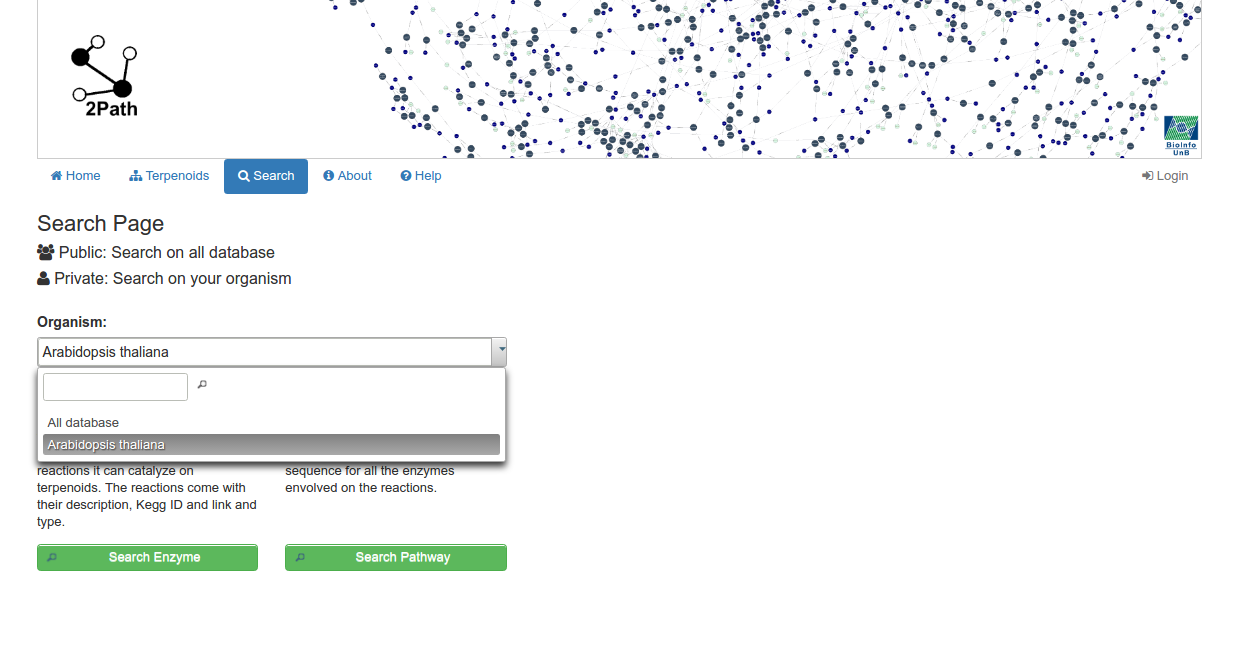
\includegraphics[width=1\textwidth]{new_search_page.png}
    \caption{Nova interface da página principal de buscas.}
    \label{fig:new_search_page}
\end{figure}

\indent A antiga interface para buscar por enzima possuia duas páginas, nas quais o objetivo da primeira era relatar se a enzima existe no banco de dados e o objetivo da segunda era de apresentar o grafo da enzima e as reações que catalisava, se existisse. Essa interface, porém era bastante confusa, principalmente os \textit{feedbacks} dados na busca, pois não atualizavam corretamente. A função de \textit{auto-complete} do EC das enzimas também diminuiu a usabilidade, pois acredita-se que não seja natural um campo de entrada completar números. Além disso, quando o usuário seguia para a página de visualização dos dados biológicos, eles precisavam clicar e arrastar os nós de maneira forçada, pois os mesmos não paravam de se mexer. O objetivo era apresentar um grafo simples e interativo, porém a experiência de usuário não correspondeu ao esperado.

\indent A nova interface para busca de enzima sofreu fortes mudanças. Não há mais função de \textit{auto-complete} no campo de entrada de EC, foi adicionado um botão para retornar à página de busca e, principalmete, o grafo aparece na mesma página. Se existe enzima, o grafo aparece, se não existe, não aparece. Os rótulos dos nós, que antes apresentavam seus nomes, agora apresenta seus identificadores no KEGG. Acima do grafo está uma legenda que aparece quando o usuário passa o \textit{mouse} por cima dos nós. Ela possui informações sobre o tipo do nó, seu nome e seu identificador no KEGG.

\indent A Figura \ref{fig:new_enzyme_4_catalyses}, além de apresentar a nova interface, mostra que não é possível representar as reações como enzimas, pois uma enzima pode catalizar mais de uma reação. Se as próprias reações possuíssem informação sobre qual enzima às catalisam, então essa mudança seria possível. Essa alteração no banco de dados facilitaria bastante a interpretação do grafo, de acordo com os biólogos, que costumaram entender reação como aresta. Por fim, a legenda do grafo ficou mais simples, portanto, mais legível.

\begin{figure}[!h]
	\centering
	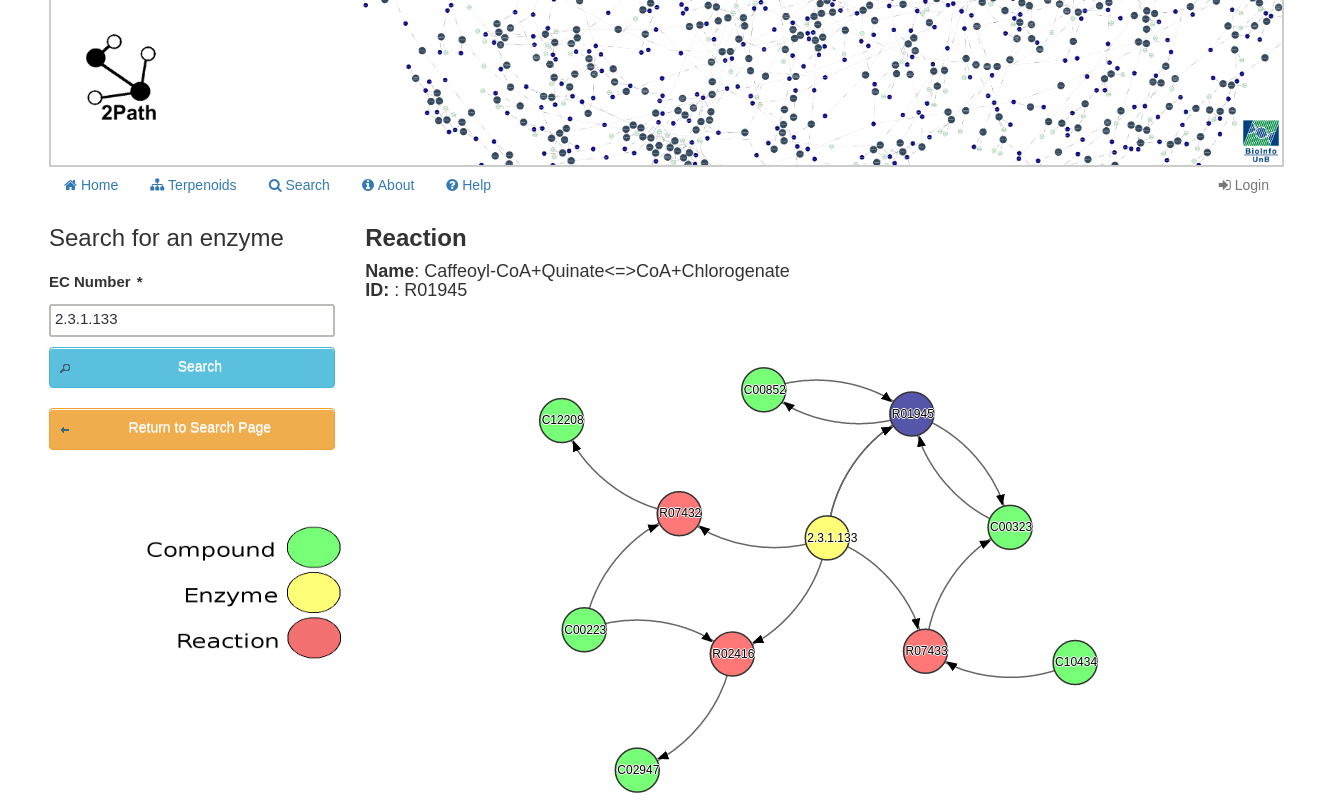
\includegraphics[width=1\textwidth]{new_enzyme_4_catalyses.png}
	\caption{Nova interface da página de busca por enzima, tanto em um organismo quanto no banco de dados completo.}
	\label{fig:new_enzyme_4_catalyses}
\end{figure}

\indent Em relação à busca por vias metabólicas, a nova interface se assemelha com a de busca por enzima, porém continua com a função de \textit{auto-complete} nos campos de entrada por nome de compostos, que foi uma boa decisão de projeto. A Figura \ref{fig:new_message_success} apresenta o resultado da busca pela via entre \textit{Caffeate} e \textit{Chlorogenate}. Observa-se que retornou sucesso, pois além de a via ter aparecido na tela, uma mensagem de sucesso aparece, por 5 segundos, no canto superior direito da tela.

\begin{figure}[!h]
    \centering
    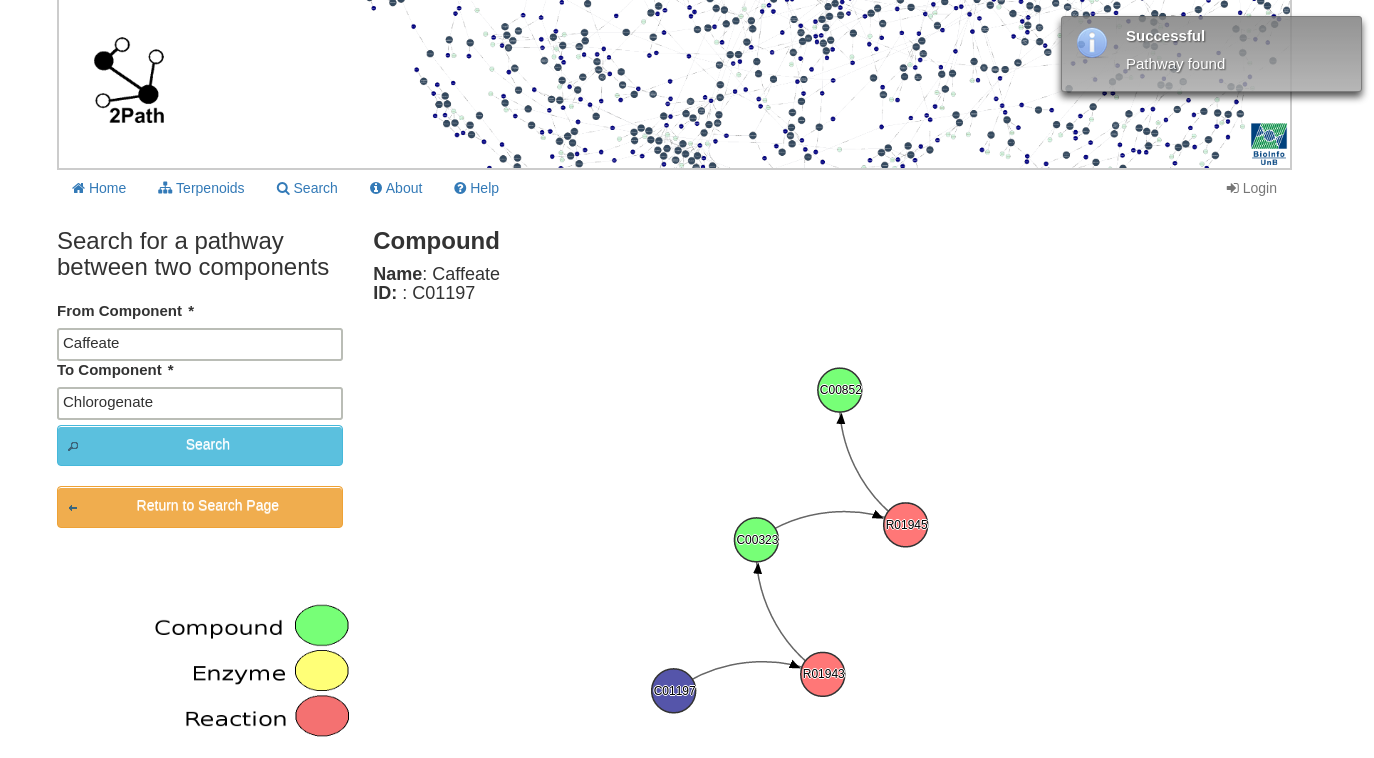
\includegraphics[width=1\textwidth]{new_message_success.png}
    \caption{Nova interface da página de busca por via metabólica, tanto em um organismo quanto no banco de dados completo. Nesse caso, a busca retornou sucesso no banco de dados completo do 2Path.}
    \label{fig:new_message_success}
\end{figure}

\indent As Figuras \ref{fig:new_message_error} e \ref{fig:new_pathway} aprensentam resultados de busca por via metabólica em um organismo. A primeira retornou falso, como visto pela mensagem de erro. A segunda retornou mensagem de sucesso e um grafo estático na tela. Observe que, apesar de a buscar ter sido no organismo, a única informação que interessa para o usuário é da via entre um composto e outro. Portanto não aparecem mais como na interface antiga os nós do organismo, sequências e enzimas. Acredita-se que essa nova decisão de projeto diminui a complexidade da visualização dos dados biológicos.

\begin{figure}[!h]
    \centering
    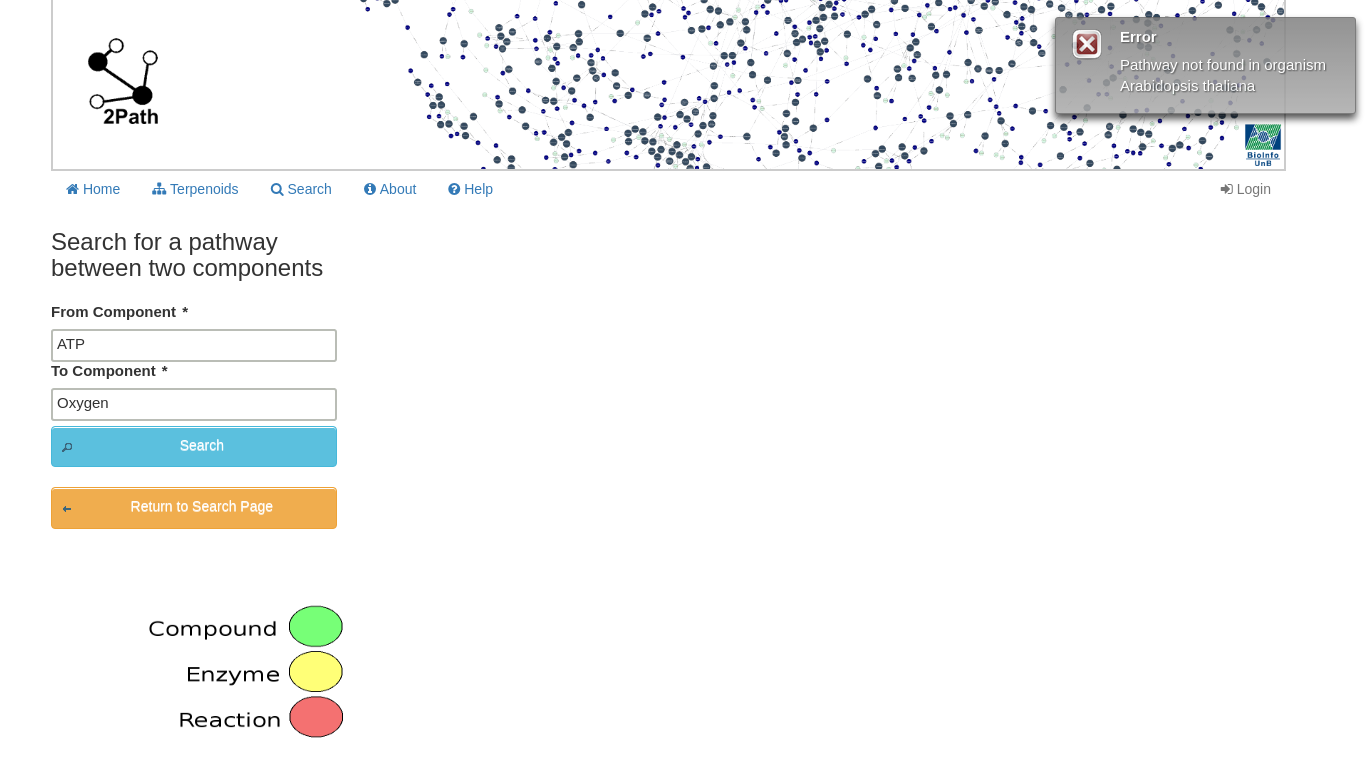
\includegraphics[width=1\textwidth]{new_message_error.png}
    \caption{Nova interface de busca por via metabólica quando a busca retorna erro de via não encontrada.}
    \label{fig:new_message_error}
\end{figure}

\newpage
\begin{figure}[!t]
    \centering
    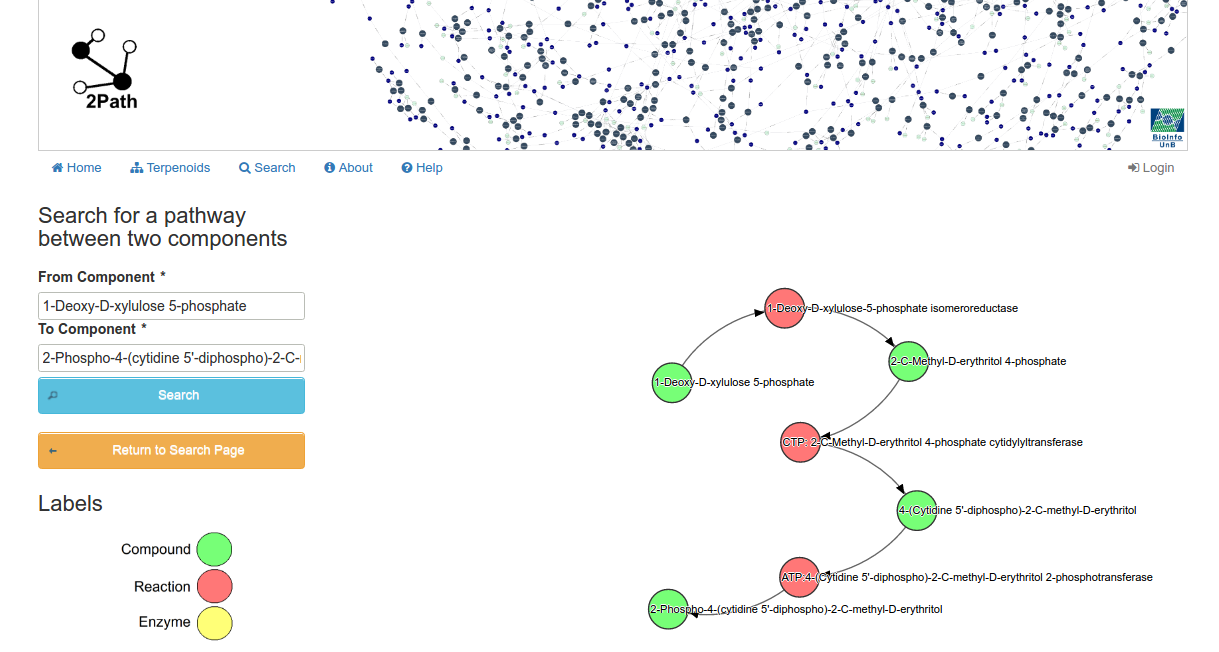
\includegraphics[width=1\textwidth]{new_pathway.png}
    \caption{Resultado de busca por via metabólica em um organismo, onde o grafo gerado possui apenas informação sobre os compostos pesquisados e as reações entre eles.}
    \label{fig:new_pathway}
\end{figure}




